\documentclass[tikz,border=2pt]{standalone}
\usepackage{amsmath}
\usetikzlibrary{arrows.meta}
\begin{document}
% One vector, two descriptions: x = (3,1)^T = 3e_1 + 1e_2 in standard coordinates and
% x = 2b_1 + 1b_2 with b_1 = (1,1)^T, b_2 = (1,-1)^T, so [x]_B = B^{-1}x = (2,1)^T.
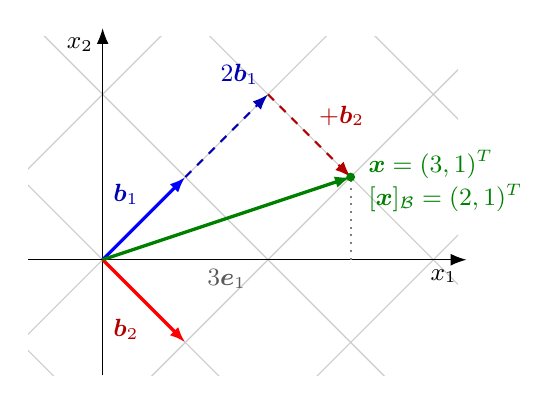
\begin{tikzpicture}[font=\small, >={Latex[length=2mm]}, x=1.05cm, y=1.05cm]
  % grid of the basis B (lines x1 + x2 = 2s and x1 - x2 = 2t)
  \begin{scope}
    \clip (-0.9,-1.4) rectangle (4.3,2.7);
    \foreach \k in {-2,...,4} {
      \draw[gray!40] ({\k-4},{\k+4}) -- ({\k+4},{\k-4});
      \draw[gray!40] ({\k-4},{-\k-4}) -- ({\k+4},{-\k+4});
    }
  \end{scope}
  % standard axes
  \draw[->] (-0.9,0) -- (4.4,0) node[below left] {$x_1$};
  \draw[->] (0,-1.4) -- (0,2.8) node[below left] {$x_2$};
  % standard description 3e_1 + e_2
  \draw[gray, thick, dotted] (3,0) -- (3,1);
  \node[gray!70!black, anchor=north] at (1.5,0) {$3\boldsymbol{e}_1$};
  % basis vectors
  \draw[->, blue, very thick] (0,0) -- (1,1);
  \node[blue!70!black, anchor=south east] at (0.55,0.55) {$\boldsymbol{b}_1$};
  \draw[->, red, very thick] (0,0) -- (1,-1);
  \node[red!70!black, anchor=north east] at (0.55,-0.6) {$\boldsymbol{b}_2$};
  % B description 2b_1 + b_2
  \draw[->, blue!70!black, thick, dashed] (1,1) -- (2,2);
  \node[blue!70!black, anchor=south east] at (2,2) {$2\boldsymbol{b}_1$};
  \draw[->, red!70!black, thick, dashed] (2,2) -- (3,1);
  \node[red!70!black, anchor=south west] at (2.5,1.5) {$+\boldsymbol{b}_2$};
  % the vector itself
  \draw[->, green!50!black, very thick] (0,0) -- (3,1);
  \fill[green!50!black] (3,1) circle (1.6pt);
  \node[green!50!black, anchor=west, align=left] at (3.1,0.95)
    {$\boldsymbol{x}=(3,1)^T$\\[1pt] $[\boldsymbol{x}]_{\mathcal B}=(2,1)^T$};
\end{tikzpicture}
\end{document}
